

\documentclass[12pt]{article}

\usepackage[margin=1in]{geometry}

% For using float option H that places figures exatcly where we want them
\usepackage{float}
% makes figure font bold
\usepackage{caption}
\captionsetup[figure]{labelfont=bf}
% For text generation
\usepackage{lipsum}
% For drawing
\usepackage{tikz}
% For smaller or equal sign and not divide sign
\usepackage{amssymb}
% For the diagonal fraction
\usepackage{xfrac}
% For enumerating exercise parts with letters instead of numbers
\usepackage{enumitem}
% For dfrac, which forces the fraction to be in display mode (large) e
% even in math mode (small)
\usepackage{amsmath}
% For degree sign
\usepackage{gensymb}
% For "\mathbb" macro
\usepackage{amsfonts}
\newcommand{\N}{\mathbb{N}}
\newcommand{\Z}{\mathbb{Z}}
\newcommand{\Q}{\mathbb{Q}}
\newcommand{\R}{\mathbb{R}}
\newcommand{\C}{\mathbb{C}}

% overline short italic
\newcommand{\olsi}[1]{\,\overline{{#1}}}
\newcommand{\ang}[1]{\langle #1 \rangle}

\usepackage{indentfirst}
\usetikzlibrary{shapes,positioning,fit,calc}

\usepackage{changepage} % for adjustwidth environment

\title{%
    \Huge Abstract Algebra \\
    \large by \\
    \Large Dummit and Foote \\~\\
    \huge Part 1: Group Theory \\
    \LARGE Chapter 2: Subgroups \\
    \Large Section 5: The Lattice of Subgroups of a Group
}
\date{2024-04-03}
\author{Michael Saba}

\begin{document}
    \pagenumbering{gobble}
    \maketitle
    \newpage
    \pagenumbering{arabic}

    
    This section introduces the concept of a graph 
    that can be used to depict the relation between groups
    and their subgroups. \\

    \subsection*{The Lattice of Subgroups}

    The \textbf{lattice of subgroups} of a group
    is a graph that illustrates the relation between
    the group and its subgroups,
    and between those subgroups and each other
    (some subgroups of the group may also be
    subgroups of other subgroups). \\
    It can be more useful to understanding the structure of a Group
    than the multiplicative table of the group is. \\
    To draw the lattice of some group $G$,
    we first start by placing the trivial group $\{1\}$
    at the bottom
    (which is always a subgroup of $G$)
    and place $G$ at the top
    (also a subgroup of itself). \\
    We then place the rest of the subgroups
    between the two.
    Generally speaking, the larger a subgroup is,
    the higher it will be, in adherence to the next rule.
    We then draw a line from a subgroup $A$ to $B$
    if $A \leqslant B$ and there are no subgroups
    properly between the two such that $A < C < B$.
    If such a group $C$ exists,
    then we instead draw the line from $A$ to $C$,
    then $C$ to $B$
    (granted there are no subgroups properly between them). \\
    This means that if we can trace a path down from subgroup $H$
    to subgroup $K$ that may or may not pass through
    other subgroups $H_1, H_2 \dots H_n$,
    then
    \[ K \leqslant H_n \leqslant H_{n-1} \leqslant \dots H_1 \leqslant H \].
    which means that $K \leqslant H$.
    So if we can trace a path from one subgroup to another,
    (always going down),
    then the subgroup we arrive to will be a subgroup
    of the subgroup we started from. \\
    Note that $G$ will be the unique subgroup at the top of the lattice
    such that it is not a subgroup of any other subgroup.
    Th trivial subgroup $\{1\}$ will be the unique
    subgroup at the bottom of the lattice,
    such that no subgroups are subgroups of it. \\
    
    We know from section 1.2.4 that 
    when $H$ and $K$ are subgroups of $G$
    (which makes them subsets of $G$),
    $\ang{H, K}$
    is the smallest subgroup containing both of them
    (their union).
    We call this the \textbf{join} of the two subgroups $H$ and $K$. \\
    To find it on the lattice,
    we can trace the path up from $H$ and $K$
    until we find the first subgroup that contains both.
    The fact that no intermediary groups exist
    between each groups connected by a line is what ensures
    this is indeed the smallest subgroup that contains both. \\
    Likewise, by a symmetric process,
    we can read the largest subgroup contained in both $H$
    and $K$ by tracing a path down from them,
    until we reach a subgroup in common between the two paths. \\

    One limit of the lattice of subgroups is that it can't
    really be drawn for infinite groups. \\

    Two lattices are said to be the same if the
    connections between elements are the same,
    even if the subgroups themselves are different
    (e.g. we focus only on the structure and paths). \\
    Two isomorphic groups obivously have the same lattices,
    but two non-isomorphic groups may also have the same lattices
    (the lattice is not unique to groups equivalent
    up to isomorphism).
    This is because lattices only carry part of the data
    that describes a group, not all of it. \\

    \subsection*{Examples of Lattices}

    For a cyclic group such as $\Z/24\Z$,
    the lattice will look like this:
    \begin{figure}[H]
        \centering
        % figure is a tikz drawing
        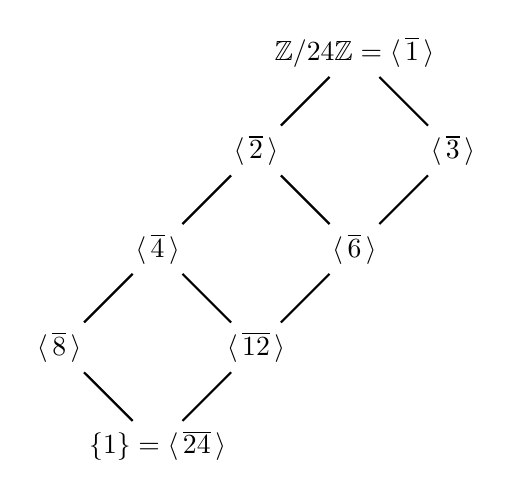
\begin{tikzpicture}[scale=2.5]
        \def\d{.4cm}
        \def\v{0cm}
        \tikzset{}
        \begin{scope}[shift={(0, 0, 0)}, rotate=0]
            \node (1) at (0, 0) {$\Z/24\Z = \ang{\olsi{1} \,}$}; 
            \node (2) at (-0.5, -0.5)
            {$\langle \olsi{2} \, \rangle$}; 
            \node (3) at (0.5, -0.5)
            {$\langle \olsi{3} \, \rangle$}; 
            \node (4) at (-1, -1)
            {$\langle \olsi{4} \, \rangle$}; 
            \node (6) at (0, -1)
            {$\langle \olsi{6} \, \rangle$}; 
            \node (8) at (-1.5, -1.5)
            {$\langle \olsi{8} \, \rangle$}; 
            \node (12) at (-0.5, -1.5)
            {$\langle \olsi{12} \, \rangle$}; 
            \node (0) at (-1, -2)
            {$\{1\} = \ang{\olsi{24} \,}$}; 
        \end{scope}

        \begin{scope}[thick]
            \draw (1) -- (2);
            \draw (1) -- (3);
            \draw (2) -- (4);
            \draw (2) -- (6);
            \draw (4) -- (8);
            \draw (4) -- (12);
            \draw (3) -- (6);
            \draw (6) -- (12);
            \draw (8) -- (0);
            \draw (12) -- (0);
        \end{scope} 

        \end{tikzpicture}
    \caption{\label{fig:figure1} Lattice of $\Z/24\Z$.}
    \end{figure} 

    The lattice of a cyclic group $Z_n$
    where $n$ is a power of some prime $p$
    on the other hand will be a straight line. \\
    This is because,
    as we know,
    the distinct subgroups of a cyclic group
    mao bijectively to the divisors of the group's order
    (where each subgroup will have that divisor as its order). 
    $Z_{p^m}$ for some positive integer $m \in \Z^+$
    has a power of a prime $p^m$ as its order.
    The only divisors of $p^m$
    are powers $p^k$ where $0 \leqslant k \leqslant m$.
    The subgroup of order $p^k$
    is the one generated by $p^{\sfrac{m}{k}}$.
    So $Z_{p^m}$ will have all of these as subgroups:
    \[ \{ \ang{1} = Z_{p^m}, \ang{p}, \ang{p^2}
    \dots \ang{p^m} = \{1\} \} \]
    By the same argument,
    $\ang{p}$ (which is really $Z_{p^{m-1}}$)
    will have these as subgroups
    \[ \{ \ang{p}, \ang{p^2}
    \dots \ang{p^m} = \{1\} \} \]
    We can repeat this argument for each subgroup $\ang{p^k}$,
    where all subgroups $\ang{p^h}$ 
    will be contained in it so long as $k \leqslant h \leqslant m$. \\
    With that said,
    the lattice will connect
    each subgroup $\ang{p^k}$ to $\ang{p^{k+1}}$,
    as it will be the only subgroup contained in it
    such that there are no intermediary subgroups between the two:
    \begin{figure}[H]
        \centering
        % figure is a tikz drawing
        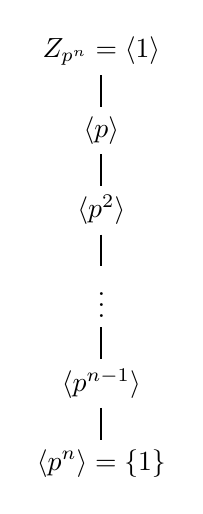
\begin{tikzpicture}[scale=2.5]

        \def\d{.4cm}

        % Specifies where the x, y coordinate of the tip of
        % the unite vectors in turn
        \tikzset{}
        
        % Scope used to shift the coordinates from the basis
        \begin{scope}[shift={(0, 0, 0)}, rotate=0]
            \node (1) at (0, 0)
            {$Z_{p^n} = \ang{1}$}; 
            \node (2) [below=\d of 1]
            {$\langle p \rangle$}; 
            \node (4) [below= \d of 2]
            {$\langle p^2 \rangle$}; 
            \node (8) [below= \d of 4]
            {$\vdots$};
            \node (16) [below= \d of 8]
            {$\ang{p^{n-1}}$}; 
            \node (0) [below= \d of 16]
            {$\ang{p^n} = \{1\}$}; 
        \end{scope}

        \begin{scope}[thick]
            \draw (1) -- (2);
            \draw (2) -- (4);
            \draw (4) -- (8);
            \draw (8) -- (16);
            \draw (16) -- (0);
        \end{scope} 

        \end{tikzpicture}
    \caption{\label{fig:figure1} Lattice of $Z_{p^n}$.}
    \end{figure} 

    The lattice of the symmetric group $S_3$ is
    \begin{figure}[H]
        \centering
        % figure is a tikz drawing
        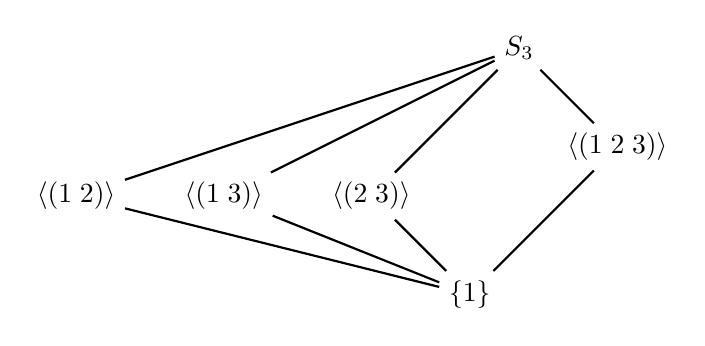
\begin{tikzpicture}[scale=2.5]

        \def\d{.5cm}

        % Specifies where the x, y coordinate of the tip of
        % the unite vectors in turn
        \tikzset{}
        
        % Scope used to shift the coordinates from the basis
        \begin{scope}[shift={(0, 0, 0)}, rotate=0]
            \node (S3) at (0, 0) {$S_3$};   
            \node (A1) at (0.5, -0.5)
            {$\langle (1\;2\;3) \rangle$}; 
            \node (B1) at (-0.75, -0.75)
            {$\langle (2\;3) \rangle$}; 
            \node (B2) at (-1.5, -0.75)
            {$\langle (1\;3) \rangle$};  
            \node (B3) at (-2.25, -0.75)
            {$\langle (1\;2) \rangle$};  

            \node (T1)  at (-0.25, -1.25)
            {$\left\{ 1 \right\}$}; 
        \end{scope}

        \begin{scope}[thick]
            \draw (S3) -- (A1);
            \draw (S3) -- (B1);
            \draw (S3) -- (B2);
            \draw (S3) -- (B3);
            \draw (A1) -- (T1);
            \draw (B1) -- (T1);
            \draw (B2) -- (T1);
            \draw (B3) -- (T1);
        \end{scope} 

        \end{tikzpicture}

        \caption{\label{fig:figure1} Lattice of $S_3$.}
    \end{figure} 

    The lattice of the group of quaternions $Q_8$ is       
    \begin{figure}[H]
        \centering
        % figure is a tikz drawing
        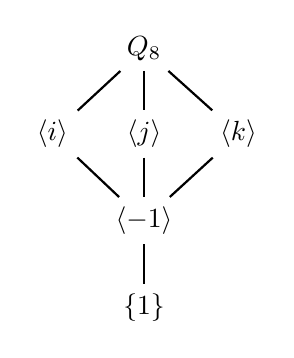
\begin{tikzpicture}[scale=2.5]

        \def\d{.5cm}

        % Specifies where the x, y coordinate of the tip of
        % the unite vectors in turn
        \tikzset{}
        
        % Scope used to shift the coordinates from the basis
        \begin{scope}[shift={(0, 0, 0)}, rotate=0]
            \node (Q8) at (0, 0) {$Q_8$};   
            \node (A1) [below left=\d and \d of Q8]
            {$\langle i \rangle$}; 
            \node (A2) [below= \d of Q8] {$\langle j \rangle$}; 
            \node (A3) [below right=\d and \d of Q8]
            {$\langle k \rangle$};  
            \node (B3) [below= \d of A2]
            {$\langle -1 \rangle$};  
            \node (T1) [below=\d of B3] {$\left\{ 1 \right\}$}; 
        \end{scope}

        \begin{scope}[thick]
            \draw (Q8) -- (A1);
            \draw (Q8) -- (A2);
            \draw (Q8) -- (A3);
            \draw (A1) -- (B3);
            \draw (A3) -- (B3);
            \draw (A2) -- (B3);
            \draw (B3) -- (T1);
        \end{scope} 

        \end{tikzpicture}
    \caption{\label{fig:figure1} Lattice of $Q_8.$}
    \end{figure} 

    The lattice of the dihedral group $D_{16}$
    \begin{figure}[H]
        \centering
        % figure is a tikz drawing
        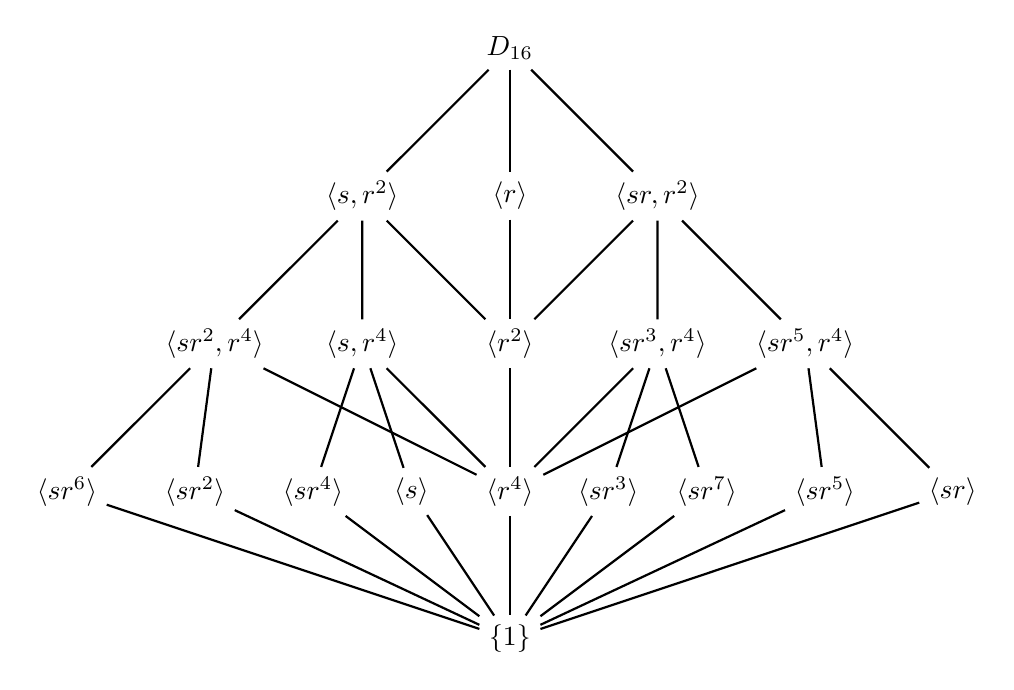
\begin{tikzpicture}[scale=2.5]

        \def\d{.8cm}
        \def\h{.6cm}

        % Specifies where the x, y coordinate of the tip of
        % the unite vectors in turn
        \tikzset{}
        
        % Scope used to shift the coordinates from the basis
        \begin{scope}[shift={(0, 0, 0)}, rotate=0]
            \node (D16) at (0, 0) {$D_{16}$};   
            \node (A1) at (-0.75, -0.75)
            {$\langle s, r^2 \rangle$}; 
            \node (A2) at (0, -0.75)
            {$\langle r \rangle$}; 
            \node (A3) at (0.75, -0.75)
            {$\langle sr, r^2 \rangle$};  
            \node (B1) at (-1.5, -1.5)
            {$\langle sr^2, r^4 \rangle$}; 
            \node (B2) at (-0.75, -1.5)
             {$\langle s, r^4 \rangle$}; 
            \node (B3) at (0, -1.5)
            {$\langle r^2 \rangle$};  
            \node (B4) at (0.75, -1.5)
            {$\langle sr^3, r^4 \rangle$}; 
            \node (B5) at (1.5, -1.5)
            {$\langle sr^5, r^4 \rangle$};  

            \node (C1) at (-2.25, -2.25)
            {$\langle sr^6 \rangle$}; 
            \node (C2) at (-1.6, -2.25)
            {$\langle sr^2 \rangle$}; 
            \node (C3) at (-1, -2.25)
            {$\langle sr^4 \rangle$}; 
            \node (C4) at (-0.5, -2.25)
            {$\langle s \rangle$}; 
            \node (C5) at (0, -2.25)
            {$\langle r^4 \rangle$};
            \node (C6) at (0.5, -2.25)
            {$\langle sr^3 \rangle$}; 
            \node (C7) at (1, -2.25)
            {$\langle sr^7 \rangle$};
            \node (C8) at (1.6, -2.25)
            {$\langle sr^5 \rangle$};  
            \node (C9) at (2.25, -2.25)
            {$\langle sr \rangle$};  
            \node (T1) at (0, -3) 
            {$\left\{ 1 \right\}$}; 
        \end{scope}

        \begin{scope}[thick]
            \draw (D16) -- (A1);
            \draw (D16) -- (A2);
            \draw (D16) -- (A3);
            \draw (A1) -- (B1);
            \draw (A1) -- (B2);
            \draw (A1) -- (B3);
            \draw (A3) -- (B5);
            \draw (A3) -- (B4);
            \draw (A3) -- (B3);
            \draw (A2) -- (B3);
            \draw (B3) -- (C5);
            \draw (B1) -- (C1);
            \draw (B1) -- (C2);
            \draw (B1) -- (C5);
            \draw (B2) -- (C3);
            \draw (B2) -- (C4);
            \draw (B2) -- (C5);
            \draw (B4) -- (C6);
            \draw (B4) -- (C7);
            \draw (B4) -- (C5);
            \draw (B5) -- (C8);
            \draw (B5) -- (C9);
            \draw (B5) -- (C5);

            \foreach\x in {1,..., 9}
            \draw (C\x) -- (T1);
        \end{scope} 

        \end{tikzpicture}

        \caption{\label{fig:figure1} Lattice of $D_{16}$.}
    \end{figure} 

    The \textbf{Klein $4$-group} or \textbf{Viergruppe},
    denoted $V_4$,
    is the group of order $4$ that has this multiplication table
    \begin{figure}[H]
        \centering

        \[\vbox{\tabskip0.5em\offinterlineskip
        \halign{\strut$#$\hfil\ \tabskip1em\vrule&&$#$\hfil\cr
        ~   & 1   & a   & b & c \cr
        \noalign{\hrule}\vrule height 12pt width 0pt
        1   & 1 & a & b & c \cr 
        a   & a & 1 & c & b \cr 
        b   & b & c & 1 & a \cr 
        c   & c & b & a & 1 \cr
        }}\]

        \caption{\label{fig:figure1} The multiplication table
        of $V_4$.}
    \end{figure}
    and it has this lattice
    \begin{figure}[H]
        \centering
        % figure is a tikz drawing
        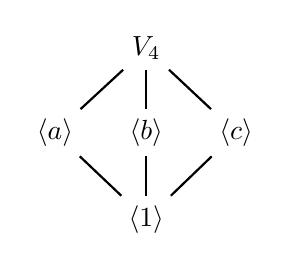
\begin{tikzpicture}[scale=2.5]

        \def\d{.5cm}

        % Specifies where the x, y coordinate of the tip of
        % the unite vectors in turn
        \tikzset{}
        
        % Scope used to shift the coordinates from the basis
        \begin{scope}[shift={(0, 0, 0)}, rotate=0]
            \node (Q8) at (0, 0) {$V_4$};   
            \node (A1) [below left=\d and \d of Q8]
            {$\langle a \rangle$}; 
            \node (A2) [below= \d of Q8] 
            {$\langle b \rangle$}; 
            \node (A3) [below right=\d and \d of Q8]
            {$\langle c \rangle$};  
            \node (B3) [below= \d of A2]
            {$\langle 1 \rangle$};  
        \end{scope}

        \begin{scope}[thick]
            \draw (Q8) -- (A1);
            \draw (Q8) -- (A2);
            \draw (Q8) -- (A3);
            \draw (A1) -- (B3);
            \draw (A3) -- (B3);
            \draw (A2) -- (B3);
        \end{scope} 

        \end{tikzpicture}
    \caption{\label{fig:figure1} Lattice of $V_4.$}
    \end{figure} 

    \subsection*{More on Lattices}
    
    Sometimes, we only care about the relationship
    between certain subgroups in the lattice.
    In that case, we can draw a \textbf{sublattice}
    of the group which only contains the groups we care about. \\
    The rules stated earlier still apply,
    where we only draw a line between subgroups
    if one is contained in the other
    and no intermediate subgroups exist between them.
    However, this only applies to subgroups that we did include
    in the sublattice;
    there may be intermediary subgroups,
    so long as they were ommited from the sublattice.
    We allow this perversion of the rules
    because we need to be able to
    trace the relationship between the subgroups
    without having to include all the subgroups. \\
    This is also useful for infinite groups,
    where drawing the full lattice is infeasible.
    As an example, this is a sublattice of $D_16$:
    \begin{figure}[H]
        \centering
        \begin{tikzpicture}[scale=2.5]
        \def\d{.5cm}
        \tikzset{}
        \begin{scope}[shift={(0, 0, 0)}, rotate=0]
            \node (Q8) at (0, 0)
            {$\ang{s, r^2}$};   
            \node (A1) at (-0.5, -0.5)
            {$\langle sr^2, r^4 \rangle$}; 
            \node (A2) at (0, 0.5)
            {$D_{16}$}; 
            \node (A3) at (0.5, -0.5)
            {$\langle r^2 \rangle$};  
            \node (B3) at (0, -1)
            {$\langle r^4 \rangle$};  
            \node (T1) at (0, -1.5)
            {$\left\{ 1 \right\}$}; 
        \end{scope}

        \begin{scope}[thick]
            \draw (Q8) -- (A1);
            \draw (Q8) -- (A2);
            \draw (Q8) -- (A3);
            \draw (A1) -- (B3);
            \draw (A3) -- (B3);
            \draw (B3) -- (T1);
        \end{scope} 

        \end{tikzpicture}
    \caption{\label{fig:figure1} A sublattice of $D_{16}$.}
    \end{figure} 

    It is easy to compute centralizers and normalizers 
    of a group given its lattice.
    This is because we know that the centralizers and normalizers
    are themselves subgroups,
    and we can use the process of elimination
    to figure out which subgroup in the lattice
    corresponds to them. \\
    For example, suppose we want to find
    the centralizer $C_{D_8}(s)$ in $D_8$.
    The lattice of $D_8$ is
    \begin{figure}[H]
        \centering
        % figure is a tikz drawing
        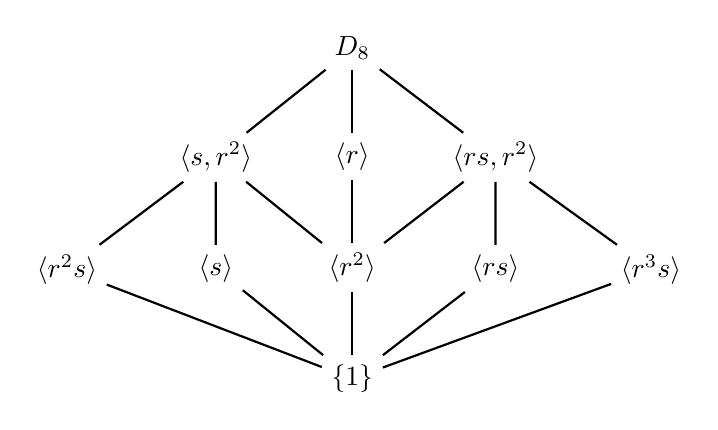
\begin{tikzpicture}[scale=2.5]

        \def\d{.8cm}

        % Specifies where the x, y coordinate of the tip of
        % the unite vectors in turn
        \tikzset{}
        
        % Scope used to shift the coordinates from the basis
        \begin{scope}[shift={(0, 0, 0)}, rotate=0]
            \node (Q8) at (0, 0) {$D_8$};   
            \node (A1) [below left=\d and \d of Q8]
            {$\langle s, r^2 \rangle$}; 
            \node (A2) [below= \d of Q8] {$\langle r \rangle$}; 
            \node (A3) [below right=\d and \d of Q8]
            {$\langle rs, r^2 \rangle$};  
            \node (B1) [below left=\d and \d of A1]
            {$\langle r^2s \rangle$}; 
            \node (B2) [below= \d of A1] {$\langle s \rangle$}; 
            \node (B3) [below= \d of A2]
            {$\langle r^2 \rangle$};  
            \node (B4) [below= \d of A3] {$\langle rs \rangle$}; 
            \node (B5) [below right=\d and \d of A3]
            {$\langle r^3s \rangle$};  
            \node (T1) [below=\d of B3] {$\left\{ 1 \right\}$}; 
        \end{scope}

        \begin{scope}[thick]
            \draw (Q8) -- (A1);
            \draw (Q8) -- (A2);
            \draw (Q8) -- (A3);
            \draw (A1) -- (B1);
            \draw (A1) -- (B2);
            \draw (A1) -- (B3);
            \draw (A3) -- (B5);
            \draw (A3) -- (B4);
            \draw (A3) -- (B3);
            \draw (A2) -- (B3);

            \foreach\x in {1,..., 5}
            \draw (B\x) -- (T1);
        \end{scope} 

        \end{tikzpicture}

        \caption{\label{fig:figure1} Lattice of $D_8$.}
    \end{figure} 
    Obviously $s$ is part of the centralizer
    as it obviously commutes with itself.
    We know that $r^2s = sr^{-2} = sr^2$ in $D_8$,
    so $r^2$ is also part of the centralizer of $s$.
    Since both of these elemets generate $\ang{s, r^2}$
    it must be that all elements in it
    (which are just a product of the two)
    commut with $s$. \\
    So $\ang{s, r^2} \leqslant C_{D_8}(s)$
    (it is a subset of the centralizer,
    and both are subgroups of $D_8$,
    so it is automatically a subgroup of the centralizer). \\
    The only subgroup that contains $\ang{s, r^2}$
    in the lattice is $D_8$ itself.
    We know it's not equal to the centralizer,
    since $r$ does not commute with $s$;
    therefore, it must be that $\ang{s, r^2} = C_{D_8}(s)$. \\


\end{document}
